\newpage
\section{Systembeschreibung im Zustandsraum}
\subsection{Allgemein (Mehrgrößensystem MIMO) }
\begin{mdframed}[style=exercise]
	\vspace{-1em}
	\begin{align*}
		\dot{\Vec{x}}(t) & = A\vec{x}(t) + B\vec{u}(t) \quad x(0) = x_{0} \\
		\vec{y}(t)       & = C\vec{x}(t) + D\vec{u}(t)
	\end{align*}
\end{mdframed}

\begin{center}
	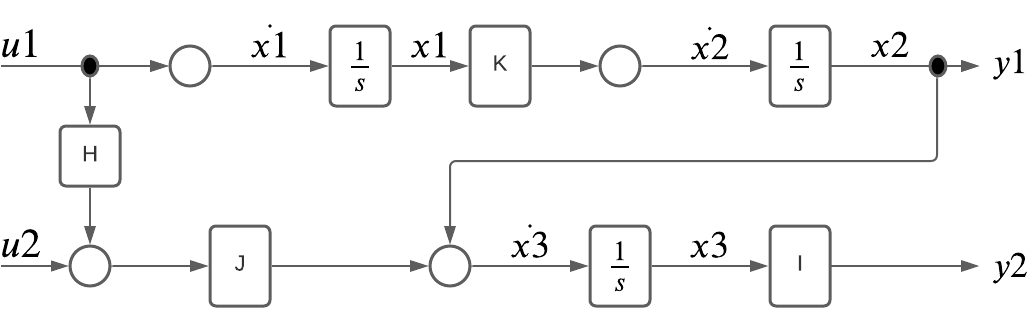
\includegraphics[width=0.96\columnwidth]{Figures/Signalflussplan.png}
	\captionof{figure}{Signalflussplan}
\end{center}

\begin{mdframed}[style=exercise]
	\begin{align*}
		\dot{x}_{1} & = 0\cdot x_{1} +0\cdot x_{2} +0\cdot x_{3} +1\cdot u_{1}+0\cdot u_{2}        \\
		\dot{x}_{2} & = K\cdot x_{1} +0\cdot x_{2} +0\cdot x_{3} +0\cdot u_{1}+0\cdot u_{2}        \\
		\dot{x}_{3} & = 0\cdot x_{1} +0\cdot x_{2} +0\cdot x_{3} +H\cdot J\cdot u_{1}+J\cdot u_{2} \\
		\dot{y}_{1} & = 0\cdot x_{1} +1+x_{2} +0\cdot x_{3} +0\cdot u_{1}+0\cdot u_{2}             \\
		\dot{y}_{2} & = 0\cdot x_{1} +0\cdot x_{2} +l\cdot x_{3} +0\cdot u_{1}+0\cdot u_{2}        \\
	\end{align*}
\end{mdframed}

\begin{mdframed}[style=exercise]
	\[
		\ A = \begin{bmatrix}
			0 & 0 & 0 \\
			K & 0 & 0 \\
			0 & 0 & 0
		\end{bmatrix}
		C = \begin{bmatrix}
			0 & 1 & 0 \\ 
			0 & 0 & l \\
		\end{bmatrix}\]
	\[B = \begin{bmatrix}
			1         & 0 \\
			0         & 0 \\
			H\cdot{}J & J
		\end{bmatrix} \
		D = \begin{bmatrix}
			0 & 0 \\
			0 & 0
		\end{bmatrix}
	\]

	Polstellen (Eigenwerte einer Matrix bestimmen):
    \[
        \operatorname{det}(A - sE)= det
		\begin{bmatrix}
			a & b \\
			c & d \\
		\end{bmatrix} = ab - cd \overset{!}{=} 0 \quad sE =\begin{bmatrix}
			s & 0 \\
			0 & s
		\end{bmatrix}
    \]
\end{mdframed}

% \subsubsection{Polfestlegung durch vollständige Zustandsrückführung}

% \centering
% \includegraphics[width=0.8\columnwidth]{Figures/Polfestlegung.png}

% \raggedright
% Durch die freie Wahl von K können alle n Pole des Systems beliebig platziert
% werden.

% Rückführungsverstärkung: von jedem X einen Pfad zur größten Ableitung
% mit Verstärkung K zeichnen. Über neue Matrix und deren determinante kann dann
% die Reglerverstärkung bestimmt werden.

% \begin{mdframed}
% \[
% 	A = \begin{bmatrix}
% 		B(a-K)
%     \end{bmatrix}
% \]
% \begin{center}
%     \footnotesize a ist vorfaktor der $\vec{x}(t)$, siehe oben.
% \end{center}
% \end{mdframed}

% dann mit der Determinante der Matrix A: K bestimmen mit den gegebenen Polen

\subsection{Programmtechnische Umsetzung}
\[F_z(z) = \frac{2z+6}{3z+4} = \frac{2xin+6xin}{3xout+4xout1}\]

\begin{lstlisting}[language=Matlab]
  while(1)
  {
      waitinterrupt(T_A); //Abtastzeit warten
      xout2 = xout1;
      xout1 = xout;
      xin2 = xin1;
      xin1 = xin;
      input(xin);
      xout = k*xout2 - j*xin1 + o*xout1;
      output(xout);
  }
\end{lstlisting}